\addchap{Foreword}

\noindent Kami na mga Kagayanen, gabaked kay na naan ta ame na isip na Kagayanen na ambaļ dili masuļat daw dili mabasa. Uļa kaugalingen na alphabet daw uļa kaugalingen na grammar. Piro, ta mga ittaw na paryo ki danen Mam Carol J. Pebley na may tagipsuson daw may kaaļam ta pagstudyo ta mga ambaļ, danen gagastos ta iran na uras daw kaaļam na iran na pastudyuan lagan ta ambaļ nay na Kagayanen. Yi na libro isya na baked na tabang ki kami na mga Kagayanen aged ame man na makita na ambaļ na Kagayanen dili nang buat-buat nang ta mga ittaw daw dili, isya man na linggwai na alin ta Dyos na Makakagaem na ta ame na lai na Kagayanen paatagan kay man ta ame na kaugalingen na ambaļ, kultura daw duma pa na ame na pwidi ipabugal man naan ta duma na mga ittaw naan ta kalibutan i. Yi man na libro baked na tabang ta mga Kagayanen o dili Kagayanen na liag magstudyo ta ambaļ na Kagayanen. Yi man na libro baked na tabang aged dason na mga hinirasyon ta mga Kagayanen magpadayon pa gid ta mag-ambaļ ta Kagayanen, dili magsalyo alin ta ambaļ na Kagayanen munta naan ta mga language of wider communication. Yi man na libro makatabang man ta pagbawi ta ambaļ na Kagayanen na dili marwad para ta mga intrisado na mga Kagayanen na liag malik o magstudyo ta ambaļ ta iran na lai. Saksi a na libro na i bunga ta lugay na pag-istar, dayad na pagpangabui duma ta mga Kagayanen daw pagstudyo naan mismo ta ame na banwa na Cagayancillo na lugar na alinan ta ame lai na mga Kagayanen. Liag ko ipaabot ake na baked na pasalamat naan ki Mam Carol J. Pebley daw Thomas E. Payne daw ta tanan na gatabang na mabuat yi na libro na parti ta \textit{A grammar of Kagayanen}.\medskip\\
\noindent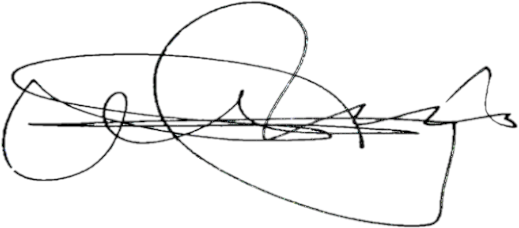
\includegraphics[width=4.5cm]{figures/mayorssignature.png}\\
\noindent Engr. \name{Sergio S.}{Tapalla} \\
\noindent Municipal Mayor\\
\noindent Municipality of Cagayancillo, Republic of the Philippines

\section*{English translation}

We the Kagayanens, we grew up having in our thinking that the Kagayanen language cannot be written and cannot be read. We didn't have our own alphabet and didn't have our own grammar. But people like Ms. Carol J. Pebley and companions who had a heart and had knowledge to study languages, they have spent their time and knowledge in studying the pattern of our Kagayanen language. This book is a big help to us the Kagayanens so that we will see that the language of Kagayanen is not just made up by people, but rather it is a language that is from Almighty God for our Kagayanen heritage, that we are given our own language, culture and other things that we should be proud of to other people in the world. Also, this book is a big help to Kagayanens and non-Kagayanens who want to study the Kagayanen language. Also, this book is a big help so that the next generations of Kagayanens will really continue to speak Kagayanen, not shift from the Kagayanen language to the languages of wider communication. Also, this book is able to help to save the Kagayanen language that it will not be lost for interested Kagayanens in returning or to studying the language of their heritage. I witness that this book is the fruit of residing a long time, maintaining good relationships with Kagayanens and studying in our very own town of Cagayancillo, the place of our Kagayanen heritage. I want to express my great thanks to Carol J. Pebley and Thomas E. Payne and all who helped in making this book about \textit{A grammar of Kagayanen}.

\section*{Information on Honorable Sergio Sembrano Tapalla Mayor of Cagayancillo, Palawan, Philippines}

Mayor Sergio S. Tapalla has been very supportive of the Kagayanen language project in many ways over a long time because of his love for his people, the Kagayanens, the culture, the language and the home island of Cagayancillo. Here are some of the things he has been involved in using his time and talents. He led a group of five who reviewed the Kagayanen translation of Genesis and the New Testament as a final step and gave very helpful feedback to improve it. He also wrote in Kagayanen about the serialized Spanish newspaper articles about Cagayancillo written in 1893 by a Spanish priest, Father \name{Salvador}{Pons}, who was parish priest in Cagayancillo for 3 years. What Mayor Tapalla wrote will be included with the English translation and other supplementary materials which have been edited by \name{Louise}{MacGregor} to be published by GPS International as an e-book, \textit{The micro-archipelago of Cagayancillo in 1893: A scholarly friar's observations}. Mayor Tapalla is also a talented musician who authored the music and lyrics of several original Kagayanen and Tagalog songs and he is the founding member of \textit{Tatos Ta Mga Kagayanen} (“Coconut Crab of the Kagayanens”) which is an all Kagayanen ethnic singing group that has performed on public stages. The songs he composed were played for a number of years on the Kagayanen radio program anchored by three Kagayanens on the local radio station GMA and currently is broadcast live via Facebook as “Kagayanen Community” which airs every Sunday evening at 8:00 pm to 9:00 pm. Many of these songs had the theme of loving the Kagayanen language and continuing to use it.

Currently (2024) Sergio S. Tapalla is the Municipal Mayor of Cagayancillo, Palawan, Philippines. He is the son of deceased former mayor of Cagayancillo \name{Atanasio A.}{Tapalla} who served undefeated in that position for 30 years. Atanasio A. Tapalla was also very supportive of the Kagayanen language project. Mayor Sergio S. Tapalla was born and grew up in Cagayancillo where he finished his elementary and high school. He is a licensed civil engineer, graduating from Central Philippines University with a Bachelor of Science in Civil Engineering in 1984. He recently retired as the City Engineer of Puerto Princesa City, Palawan. 
